%%%%%%%%%%%%%%%%%%%%%%%%%%%%%%%%%%%%%%%%%
%
% (c) 2019 by Jennifer Laaser
%
% This work is licensed under the Creative Commons Attribution-NonCommercial-ShareAlike 4.0 International License. To view a copy of this license, visit http://creativecommons.org/licenses/by-nc-sa/4.0/ or send a letter to Creative Commons, PO Box 1866, Mountain View, CA 94042, USA.
%
% The current source for these materials is accessible on Github: https://github.com/jlaaser/pogil-polymers
%
%%%%%%%%%%%%%%%%%%%%%%%%%%%%%%%%%%%%%%%%%

\renewcommand{\figpath}{content/polymchem/networks/network-synth/figs}
\renewcommand{\labelbase}{network-synth}

\begin{activity}[Synthesis of Polymer Networks]

\begin{instructornotes}
	This activity introduces students to concepts related to the synthesis of polymer networks.
	
	After completing this activity, students will be able to:
	\begin{enumerate}
		\item \dots
	\end{enumerate}
	
	\subsection*{Activity summary:}
	\begin{itemize}
		\item \textbf{Activity type:} Learning Cycle
		\item \textbf{Content goals:} Synthesis of Polymer Networks
		\item \textbf{Process goals:} %https://pogil.org/uploads/attachments/cj54b5yts006cklx4hh758htf-process-skills-official-pogil-list-2015-original.pdf
			written communication, critical thinking, information processing
		\item \textbf{Duration:} TBD
		\item \textbf{Instructor preparation required:} none beyond knowledge of relevant content
		\item \textbf{Related textbook chapters:}
			\begin{itemize}
				\item \emph{Polymer Chemistry} (Hiemenz \& Lodge): section NNN
			\end{itemize}
		%\item \textbf{Facilitation notes:}
		%	\begin{itemize}
		%		\item \dots
		%	\end{itemize}
	\end{itemize}
	
\end{instructornotes}


\begin{model}[Linking Polymer Strands]
	\label{\labelbase:mdl:linking}

	One way to synthesize a polymer network is to crosslink pre-formed polymer chains.
	
	Consider the following collection of polymer chains:
	
	\centerline{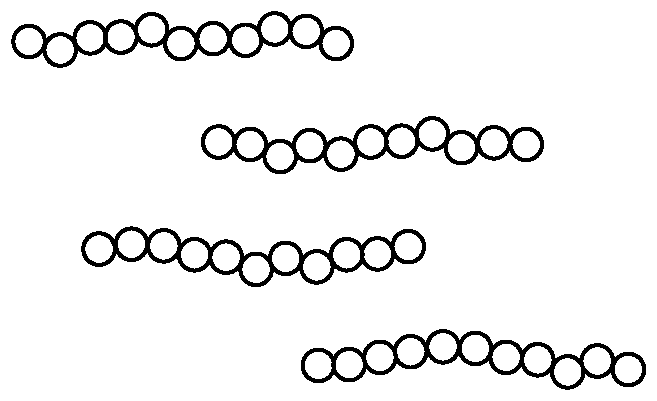
\includegraphics[width=0.5\textwidth]{\figpath/Model1_linking_blank.pdf}}
	
	To form a network, the chains must be crosslinked together to form a single large molecule:
	
	\centerline{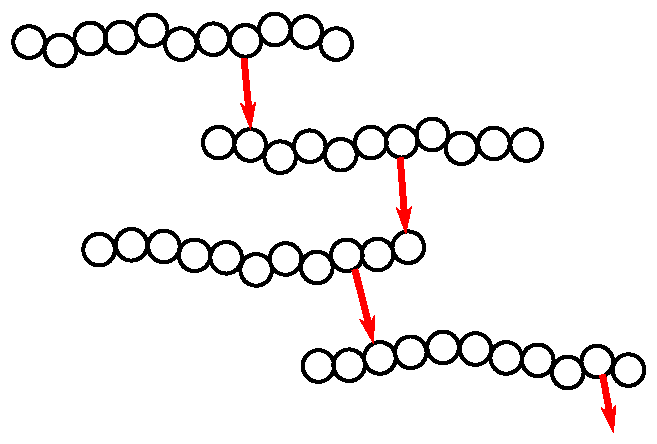
\includegraphics[width=0.5\textwidth]{\figpath/Model1_linking_arrows.pdf}}
	
	Here, we have drawn the crosslinks as arrows to make the analysis easier, but in practice, crosslinks do not have a specific orientation.
	
\end{model}


\begin{ctqs}

	\question In the picture shown in Model \ref{\labelbase:mdl:linking}, what is the \emph{minimum} number of ``outgoing'' crosslinks (arrows pointing away from the chain) that each polymer chain must have in order to allow a network to form?
	
		\begin{solution}[0.5in]
		
			one (each strand must link to the next to link all of the strands into a single molecule)
			
		\end{solution}
		
	\question If each polymer chain has $N$ monomers, what is the \emph{minimum fraction} of monomers, $x_c$, that must form an outgoing crosslink in order for a network to form?
	
		\begin{solution}[0.5in]
			$x_c = \frac{1}{N}$
		\end{solution}
		
	\question Briefly describe, in 2-3 complete sentences, how you could determine the minimum amount of crosslinker necessary to form a network from a polymer with molecular weight $M_n$.
	
		\begin{solution}[2in]
			First, take the molecular weight and divide by the monomer mass $M_0$ to find the degree of polymerization $N$.  Then, calculate the minimum fraction of monomers that need to be crosslinked to form a network using $x_c = \frac{1}{N_n}$.  Finally, use the total mass (or total number of moles) of monomer to calculate the total mass (or total number of moles) of crosslinker corresponding to this fraction.
		\end{solution}
		
	%\question Suppose a fraction $x > x_c$ of the monomers form outgoing crosslinks.
	
	%	\begin{enumerate}
	%		\item On average, how many monomers do you expect to find between outgoing crosslinks?
			
	%		\item On average, how many ``incoming'' crosslinks will that same set of monomers have?
	%		
	%		\item On average, 
	%	\end{enumerate}
	
\end{ctqs}

\begin{model}[Step-Growth Network Synthesis]

	A second way to synthesize a network is via step-growth polymerization of multi-functional monomers.
	
	For example, a step-growth polymerization of a difunctional ``AA'' monomer with a trifunctional ``B$_3$'' monomer might yield a network as follows:
	
	\centerline{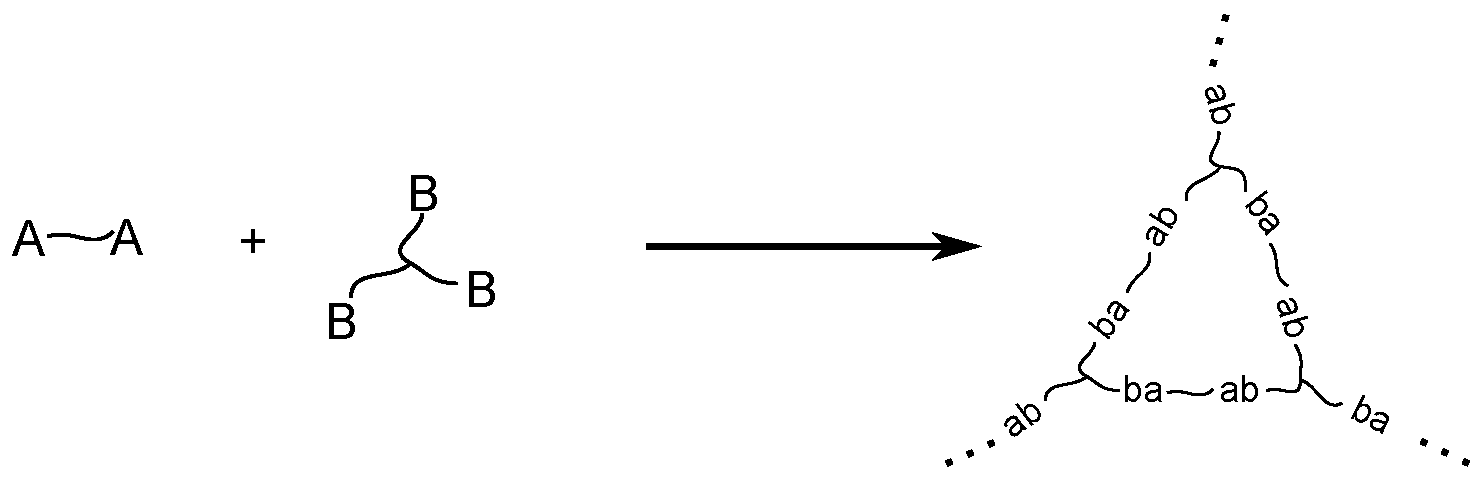
\includegraphics[width=0.7\textwidth]{\figpath/Model2_A2B3network.pdf}}

\end{model}

\begin{ctqs}

	\question Suppose that you started this reaction with 3 AA-type monomers and 2 $B_3$ monomers, as shown below:
	
	\vspace{6pt}
		\centerline{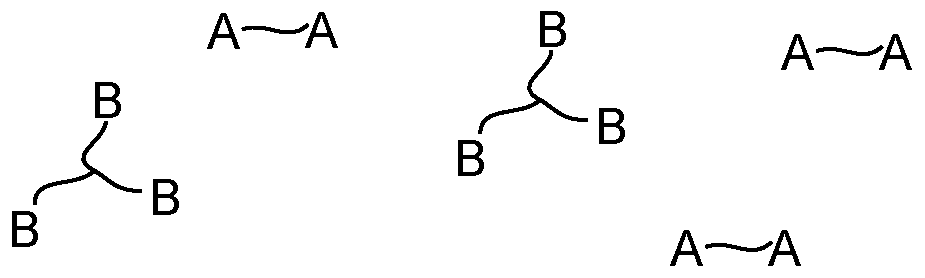
\includegraphics[width=0.5\textwidth]{\figpath/Model2_A2B3_initial.pdf}}
	
		\begin{enumerate}
			\item How many \emph{molecules} are present in the initial reaction mixture?
			
				\begin{solution}[0.75in]
					5
				\end{solution}
			
			\item How many \emph{reactive functional groups} are present in the initial reaction mixture?  For the purposes of this question, count both the A and B reactive groups.
			
				\begin{solution}[0.5in]
					12 (6 from AA-type monomers, 6 from B3-type monomers)
				\end{solution}
			
		\end{enumerate}
		
	\question Now, suppose we move two ``steps'' forward in the reaction (i.e. we form two ``ab'' bonds).
	
		\begin{enumerate}
		
			\item Draw one possible structure that could occur after two bond-forming reactions have taken place:
			
				\begin{solution}[1.75in]
				
					(student answers may vary)
					
				\end{solution}
			
			\item How many \emph{molecules} are present after two bond-forming reactions have taken place?
			
				\begin{solution}[0.5in]
					3
				\end{solution}
			
			\item How many functional groups \emph{have reacted} after two bond-forming reactions have taken place?  For the purposes of this question count both the a's and the b's.
			
				\begin{solution}[0.5in]
					4
				\end{solution}
				
			\item Calculate the extent of reaction, $p$ (fraction of functional groups that have reacted), and the number-average degree of polymerization, $N_n$, for this state of the reaction.
			
				\begin{solution}[2.25in]
					$p = \frac{\text{\# reacted}}{\text{initial \# of reactive groups}} = \frac{4}{12} = 0.33$
					
					$N_n = \frac{\text{initial \# of molecules}}{\text{final \# of molecules}} = \frac{5}{3} = 1.67$
					
					Note: students may get stuck on $N_n$.  Give them a hint if necessary.
				\end{solution}
		\end{enumerate}

	\question More generally, suppose that you initially have $n_0$ molecules that have an average of $\langle f\rangle$ reactive groups per monomer.  
	
		What is the \emph{total number} of reactive functional groups at the start of your reaction?
	
			\begin{solution}[1in]
				$n_0 \langle f \rangle$
			\end{solution}
			
	\question Suppose that at some time later, there are $n$ molecules in the reaction mixture.
	
		\begin{enumerate}
		
			\item How many bond-forming reactions must have occurred to reach this point?  \emph{(Hint: how much does the number of molecules in the reaction change each time a bond-forming reaction happens?)}
			
				\begin{solution}[0.65in]
					$n_0 - n$ (each bond-forming reaction reduces the number of molecules by one, so if we have dropped from $n_0$ to $n$ molecules, we must have undergone $n_0-n$ bond-forming reactions)
				\end{solution}
		
			\item How many functional groups must have reacted to reach this point?
			
				\begin{solution}[0.65in]
					$2(n_0-n)$ (each bond-forming reaction uses up two reactive groups)
				\end{solution}
			
			\question What is the number-average degree of polymerization at this point in the reaction?
			
				\begin{solution}[0.65in]
					$N_n = \frac{n_0}{n}$
				\end{solution}
			
			\question What is the extent of reaction at this point in the reaction?
			
				\begin{solution}[0.65in]
					$p = \frac{2(n_0-n)}{n_0\langle f \rangle}$
				\end{solution}
		
		\end{enumerate}
	
\end{ctqs}

\begin{infobox}
	Combining the expressions you derived for $p$ and $N_n$, above, it is possible to show that
	\begin{equation*}
		N_n = \frac{2}{2-p\langle f \rangle}
	\end{equation*}
	This relationship is referred to as the \emph{Carothers equation}.
\end{infobox}

\begin{ctqs}
	\question As the network begins to form, all of the monomers effectively link into a single large molecule.  What must happen to $N_n$ in this case?  Briefly explain your group's reasoning in 1-2 complete sentences.
	
		\begin{solution}[2in]
			As the monomers all link into a single molecule, $N_n$ must become very large.  In the limit of having a large number of initial monomers, $N_n$ effectively goes to infinity.
			
			\emph{Note: strictly speaking, it is actually $N_w$ that must approach infinity, but this distinction is a subtle point and not necessary for this activity.}
		\end{solution}
	
	\question What must be true about the value of $2-p\langle f \rangle$ in order for $N_n\to\infty$?
	
		\begin{solution}[1.5in]
			$2-p\langle f\rangle = 0$ (value of the fraction blows up if the denominator is zero)
		\end{solution}
	
	\question Rearrange your answer to the previous question to find the minimum extent of reaction at which a network will form.
	
		\begin{solution}[1in]
			$p = \frac{2}{\langle f \rangle}$
		\end{solution}
\end{ctqs}


\begin{exercises}

%	\exercise Exercise about stoichiometric imbalance in network synthesis?
	
	%\exercise In Model \ref{\labelbase:mdl:linking}, you considered formation of networks by linking together pre-formed polymer chains.  However, the same analysis can be used to understand networks formed by chain-growth polymerization of mixtures containing difunctional monomers.
	
	%	\begin{enumerate}
	%		\item 
	%	\end{enuemrate}	
	
	\exercise Consider the AA+BB-type step-growth polymerizations that you learned about earlier this term.
	
		\begin{enumerate}
			\item In an AA+BB-type polymerization, what is the average number of reactive functional groups per molecule?
			
			\item Show that, with this value of $\langle f\rangle$, the Carothers equation simplifies to the version you learned for step-growth polymerizations.
		\end{enumerate}	
	
\end{exercises}


%\begin{problems}
%
%	\problem First exercise
%	\problem Second exercise
%	
%\end{problems}


	
\end{activity}